\section{Propagation Delays and Transition Times}

\subsection{Propagation Delay}

The propagation delay $T_P$ is defined as the time delay between
the 50\% crossing of the input and the corresponding 50\%
crossing of the output. There are two kinds:

\begin{itemize}
    \item[$t_{pHL}$:] The time between an input change and the corresponding output change
          when the output is changing from HIGH to LOW.
    \item[$t_{pLH}$:] The time between an input change and the corresponding output change
          when the output is changing from LOW to HIGH.
\end{itemize}

\begin{figure}
    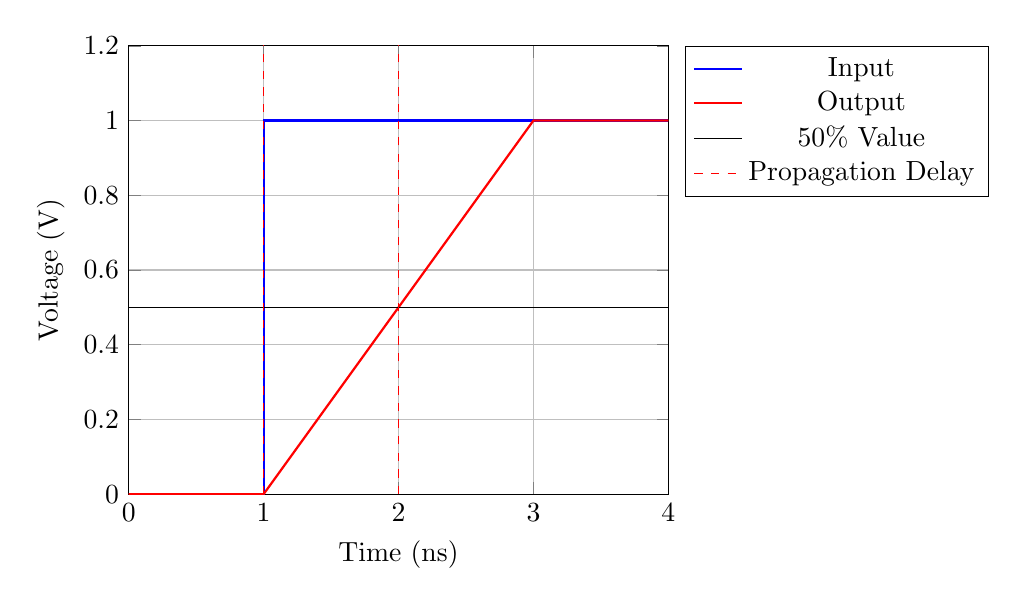
\begin{tikzpicture}
        \begin{axis}[
                xlabel={Time (ns)},
                ylabel={Voltage (V)},
                xmin=0, xmax=4,
                ymin=0, ymax=1.2,
                grid=both,
                legend pos=outer north east,
            ]
            % Input signal (step function)
            \addplot[blue, thick] coordinates {
                    (0,0) (1,0) (1,1) (4,1)
                };
            \addlegendentry{Input}

            % Output signal (delayed rise)
            \addplot[red, thick] coordinates {
                    (0,0) (1,0) (3,1) (4,1)
                };
            \addlegendentry{Output}

            % 50% crossing markers
            \addplot[mark=none, black, samples=2] {0.5};
            \addlegendentry{50\% Value}

            % 50% time delay
            \addplot +[mark=none, red, dashed] coordinates {(2, 0) (2, 2)};
            \addplot +[mark=none, red, dashed] coordinates {(1, 0) (1, 2)};
            \addlegendentry{Propagation Delay}
        \end{axis}
    \end{tikzpicture}
    \caption{Propagation Delay}
    \label{fig:propagationdelay}
\end{figure}

\subsection{Transition Time}

The amount of time that the output of a logic circuit
takes to change from one
state to another is called the transition time.
An output takes a certain time, called the rise time
($t_r$), to change from LOW to HIGH, and a
possibly different time, called the fall
time ($t_f$), to change from HIGH to LOW.
The rise time and fall time of the output signal are defined as the time
required for the voltage to change from its 10\% level to its 90\% level
or vice versa.

\begin{figure}
    \centering
    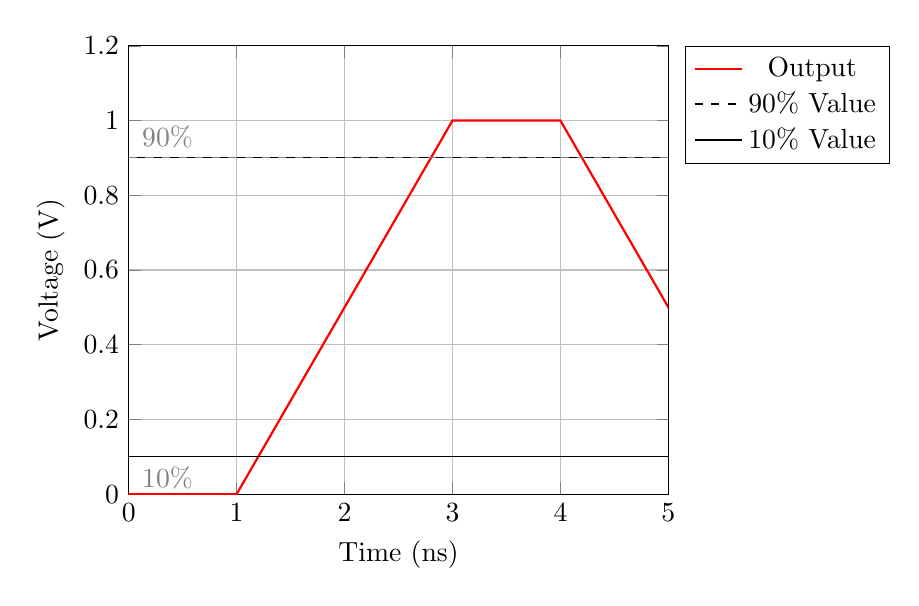
\begin{tikzpicture}
        \begin{axis}[
                xlabel={Time (ns)},
                ylabel={Voltage (V)},
                xmin=0, xmax=5,
                ymin=0, ymax=1.2,
                grid=both,
                legend pos=outer north east,
            ]
            % Output signal with rise/fall transitions
            \addplot[red, thick] coordinates {
                    (0,0) (1,0) (3,1) (4,1) (6,0)
                };
            \addlegendentry{Output}

            % Reference levels
            \draw[dashed, gray] (0,0.1) -| (6,0.1) node[pos=0.03, below] {10\%};
            \draw[dashed, gray] (0,0.9) -| (6,0.9) node[pos=0.03, above] {90\%};

            % Rise time annotation
            \addplot[mark=none, dashed, samples=2] {0.9};
            \addlegendentry{90\% Value}

            % Fall time annotation
            \addplot[mark=none, black, samples=2] {0.1};
            \addlegendentry{10\% Value}

        \end{axis}
    \end{tikzpicture}
    \label{Rise and Fall Time}
    \caption{fig:risefalltime}
\end{figure}